% =====================================================================
% IBFE Tutorials: pipe flow and transition to turbulence
% =====================================================================
\documentclass[aspectratio=169,11pt]{beamer}

% Match the visual language of the SIAM Waves talk.
\usetheme{Boadilla}
\usecolortheme{seahorse}
\useinnertheme{rectangles}
\useoutertheme{infolines}

\setbeamercolor{structure}{fg=blue!55!black}
\setbeamercolor{title}{fg=white,bg=blue!55!black}
\setbeamercolor{frametitle}{fg=blue!55!black}
\setbeamercolor{block title}{bg=blue!12,fg=blue!55!black}
\setbeamercolor{block body}{bg=blue!4}
\setbeamertemplate{navigation symbols}{}
\setbeamerfont{frametitle}{series=\bfseries,size=\large}
\setbeamerfont{title}{series=\bfseries,size=\Large}

\usepackage[T1]{fontenc}
\usepackage[utf8]{inputenc}
\DeclareFontShape{T1}{cmss}{b}{n}{<->ssub*cmss/bx/n}{}
\usepackage{amsmath,amssymb,bm,mathtools}
\usepackage{booktabs}
\usepackage{array}
\usepackage{xcolor}
\usepackage{tikz}
\usetikzlibrary{arrows.meta,calc,positioning,patterns,decorations.pathmorphing}
\usepackage{tcolorbox}
\tcbuselibrary{skins}
\usepackage{hyperref}

\hypersetup{colorlinks=true,urlcolor=blue!55!black}

\definecolor{pipeblue}{RGB}{38,86,145}
\definecolor{pipeorange}{RGB}{208,112,44}
\definecolor{pipegreen}{RGB}{53,128,95}
\definecolor{pipegray}{RGB}{92,101,112}

\newcommand{\hi}[1]{\textcolor{blue!55!black}{\textbf{#1}}}
\newcommand{\soft}[1]{\textcolor{gray!55!black}{#1}}
\newcommand{\Rey}{\mathrm{Re}}
\newcommand{\De}{\mathrm{De}}
\newcommand{\uu}{\bm{u}}
\newcommand{\qv}{\bm{q}}
\newcommand{\xvec}{\bm{x}}
\newcommand{\mean}[1]{\overline{#1}}
\newcolumntype{L}[1]{>{\raggedright\arraybackslash}p{#1}}

\newtcolorbox{punchbox}{
  enhanced,
  colback=blue!4,
  colframe=blue!55!black,
  boxrule=0.6pt,
  arc=2pt,
  left=4pt,right=4pt,top=3pt,bottom=3pt
}

\title[Pipe transition]{Pipe flow and transition to turbulence}
\subtitle{A controlled baseline for thinking about aortic flow}
\author[Miller]{Laura A. Miller}
\institute[UArizona]{Department of Mathematics, University of Arizona}
\date{}

\begin{document}

% ----- 1. Title -----
\begin{frame}[plain]
  \begin{beamercolorbox}[sep=10pt,center]{title}
    {\bfseries\Large Pipe flow and transition to turbulence}\\[3pt]
    {\normalsize A controlled baseline for thinking about aortic flow}
  \end{beamercolorbox}
  \vspace{1.0em}
  \begin{columns}[T,onlytextwidth]
  \begin{column}{0.54\textwidth}
    \textbf{\large Laura A. Miller}\\[4pt]
    Department of Mathematics\\
    University of Arizona\\[10pt]
    {\small IBFE Tutorials}\\[9pt]
    \parbox{0.96\linewidth}{\tiny AI tools were used to assist with formatting, organization, and clarification of the instructor's original notes.}
  \end{column}
  \begin{column}{0.43\textwidth}
    \begin{punchbox}
    \centering
    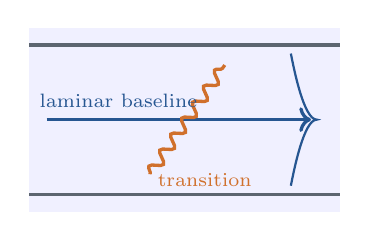
\begin{tikzpicture}[x=0.73cm,y=0.73cm]
      \fill[blue!6] (0,0) rectangle (5.4,3.2);
      \draw[very thick,pipegray] (0,0.3)--(5.4,0.3);
      \draw[very thick,pipegray] (0,2.9)--(5.4,2.9);
      \draw[pipeblue,very thick,->] (0.3,1.6)--(4.9,1.6);
      \draw[pipeblue,thick] (4.55,0.45) parabola bend (5.0,1.6) (4.55,2.75);
      \draw[decorate,decoration={snake,amplitude=2pt,segment length=7pt},pipeorange,very thick] (2.1,0.65)--(3.4,2.55);
      \node[pipeblue] at (1.55,1.92){\scriptsize laminar baseline};
      \node[pipeorange] at (3.05,0.55){\scriptsize transition};
    \end{tikzpicture}
    \end{punchbox}
  \end{column}
  \end{columns}
\end{frame}

% ----- 2. Roadmap -----
\begin{frame}{From a solvable baseline to aortic complexity}
\begin{enumerate}\itemsep7pt
  \item Derive Hagen--Poiseuille flow and audit every sign in $\Delta p$, $Q$, and wall shear.
  \item Nondimensionalize with $\Rey_D$ and distinguish laminar drag from turbulent statistics.
  \item Reconcile modal stability with transient growth and finite-amplitude transition.
  \item Read puffs, slugs, decay, and splitting in space--time.
  \item Add pulsatility, curvature, branching, compliance, and inflow disturbances.
\end{enumerate}

\begin{punchbox}
\centering
The straight rigid pipe is a reference problem. Its transition thresholds do \emph{not} transfer directly to the aorta.
\end{punchbox}
\end{frame}

% ----- 3. Coordinates -----
\begin{frame}{Fix the geometry and Reynolds-number convention}
\begin{columns}[T,onlytextwidth]
\begin{column}{0.48\textwidth}
Use cylindrical coordinates $(z,r,\theta)$ with
\[
  D=2R,
  \qquad \nu=\frac{\mu}{\rho},
\]
\[
  \Rey_D:=\frac{U_bD}{\nu}
  =\frac{\rho U_bD}{\mu}.
\]
Here $U_b=Q/(\pi R^2)$ is the bulk velocity.

\begin{block}{Why the subscript matters}
Pipe-transition references also use radius, centerline velocity, or friction velocity. State the convention before quoting a Reynolds number.
\end{block}
\end{column}
\begin{column}{0.49\textwidth}
\centering
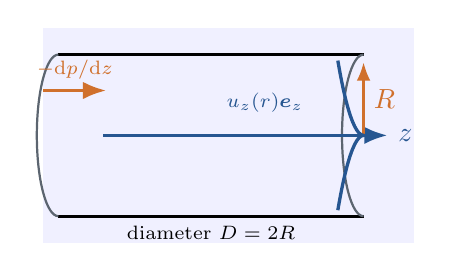
\begin{tikzpicture}[x=0.76cm,y=0.76cm,>=Latex]
  \fill[blue!6] (0,0) rectangle (6.2,3.6);
  \draw[very thick] (0.25,0.45)--(5.35,0.45);
  \draw[very thick] (0.25,3.15)--(5.35,3.15);
  \draw[pipegray,thick] (0.25,0.45) arc[start angle=270,end angle=90,x radius=0.36,y radius=1.35];
  \draw[pipegray,thick] (5.35,0.45) arc[start angle=270,end angle=90,x radius=0.36,y radius=1.35];
  \draw[->,very thick,pipeblue] (1.0,1.8)--(5.75,1.8) node[right]{$z$};
  \draw[->,thick,pipeorange] (5.35,1.8)--(5.35,3.02) node[midway,right]{$R$};
  \draw[pipeblue,very thick] (4.92,0.55) parabola bend (5.35,1.8) (4.92,3.05);
  \node[pipeblue] at (3.7,2.35){\scriptsize $u_z(r)\bm e_z$};
  \node at (2.8,0.18){\scriptsize diameter $D=2R$};
  \draw[->,pipeorange,very thick] (0.0,2.55)--(1.05,2.55) node[midway,above]{\scriptsize $-\mathrm dp/\mathrm dz$};
\end{tikzpicture}
\end{column}
\end{columns}
\end{frame}

% ----- 4. Assumptions -----
\begin{frame}{The laminar baseline is deliberately restrictive}
\begin{columns}[T,onlytextwidth]
\begin{column}{0.48\textwidth}
\begin{block}{Straight-pipe model}
\begin{itemize}\itemsep3pt
  \item incompressible, Newtonian, constant $\rho,\mu$;
  \item rigid, circular, straight wall;
  \item no slip;
  \item steady, axisymmetric, fully developed flow.
\end{itemize}
\end{block}
\end{column}
\begin{column}{0.48\textwidth}
\begin{alertblock}{Aortic departures}
\begin{itemize}\itemsep3pt
  \item pulsatile forcing and finite entrance length;
  \item curvature, branches, taper, noncircular sections;
  \item compliant, prestressed, anisotropic wall;
  \item valve jet, swirl, and upstream disturbances.
\end{itemize}
\end{alertblock}
\end{column}
\end{columns}

\vspace{0.5em}
\hi{Strategy:} derive the reference solution exactly, then identify which omitted mechanism changes each conclusion.
\end{frame}

% ----- 5. Navier--Stokes -----
\begin{frame}{Start from dimensional incompressible Navier--Stokes}
\begin{align*}
  \rho\left(\partial_t\uu+(\uu\cdot\nabla)\uu\right)
  &= -\nabla p+\mu\nabla^2\uu,\\
  \nabla\cdot\uu&=0.
\end{align*}

\begin{columns}[T,onlytextwidth]
\begin{column}{0.47\textwidth}
\begin{block}{Inertial terms}
$\rho\partial_t\uu$ is local acceleration; $\rho(\uu\cdot\nabla)\uu$ is nonlinear convection.
\end{block}
\end{column}
\begin{column}{0.49\textwidth}
\begin{block}{Forcing and diffusion}
$-\nabla p$ drives the flow; $\mu\nabla^2\uu$ diffuses momentum.
\end{block}
\end{column}
\end{columns}

Density is constant here, and no body force is included. Gravity can be absorbed into a modified pressure when appropriate.
\end{frame}

% ----- 6. Reduction -----
\begin{frame}{Fully developed symmetry removes the nonlinear term}
Take
\[
  \uu=u_z(r)\bm e_z,
  \qquad
  \partial_tu_z=\partial_zu_z=\partial_\theta u_z=0.
\]
Continuity is automatic, and $(\uu\cdot\nabla)\uu=u_z\partial_z(u_z\bm e_z)=\bm0$.

The axial momentum equation becomes
\[
  0=-\frac{\mathrm dp}{\mathrm dz}
    +\mu\frac1r\frac{\mathrm d}{\mathrm dr}
      \left(r\frac{\mathrm du_z}{\mathrm dr}\right).
\]

\begin{punchbox}
For a constant pressure drop, $\mathrm dp/\mathrm dz<0$. Define the positive driving gradient $g:=-\mathrm dp/\mathrm dz>0$.
\end{punchbox}
\end{frame}

% ----- 7. ODE and BC -----
\begin{frame}{Integrate the radial ODE with two physical conditions}
With $g=-\mathrm dp/\mathrm dz$,
\[
  \frac1r\frac{\mathrm d}{\mathrm dr}\left(r\frac{\mathrm du_z}{\mathrm dr}\right)
  =-\frac g\mu.
\]
Integrating once gives
\[
  r\frac{\mathrm du_z}{\mathrm dr}=-\frac{g}{2\mu}r^2+C_1.
\]

\begin{columns}[T,onlytextwidth]
\begin{column}{0.48\textwidth}
\begin{block}{Regularity at the centerline}
$u_z'(0)=0$ and boundedness force $C_1=0$.
\end{block}
\end{column}
\begin{column}{0.48\textwidth}
\begin{block}{No slip at the wall}
$u_z(R)=0$ determines the remaining constant.
\end{block}
\end{column}
\end{columns}
\end{frame}

% ----- 8. Profile -----
\begin{frame}{Hagen--Poiseuille flow is parabolic}
\begin{columns}[T,onlytextwidth]
\begin{column}{0.53\textwidth}
\[
  \boxed{u_z(r)=\frac{g}{4\mu}(R^2-r^2)}.
\]
Checks:
\begin{itemize}\itemsep4pt
  \item $u_z(R)=0$ and $u_z'(0)=0$;
  \item $u_z(r)\ge0$ because $g>0$;
  \item $u_z''<0$: the centerline is the maximum;
  \item units: $[gR^2/\mu]=L/T$.
\end{itemize}
\end{column}
\begin{column}{0.44\textwidth}
\centering
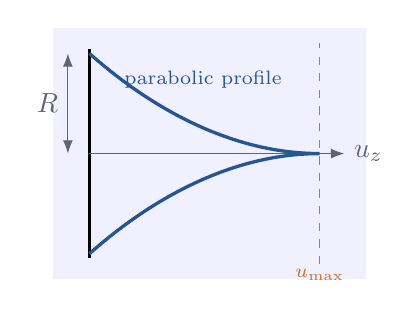
\begin{tikzpicture}[x=0.78cm,y=0.78cm,>=Latex]
  \fill[blue!6] (0,0) rectangle (5.1,4.1);
  \draw[very thick] (0.6,0.35)--(0.6,3.75);
  \draw[->,pipegray] (0.6,2.05)--(4.75,2.05) node[right]{$u_z$};
  \draw[pipeblue,very thick] (0.6,0.42) parabola bend (4.35,2.05) (0.6,3.68);
  \draw[dashed,pipeorange] (4.35,0.25)--(4.35,3.85);
  \node[pipeorange] at (4.35,0.08){\scriptsize $u_{\max}$};
  \draw[<->,pipegray] (0.25,2.05)--(0.25,3.68) node[midway,left]{$R$};
  \node[pipeblue] at (2.45,3.25){\scriptsize parabolic profile};
\end{tikzpicture}
\end{column}
\end{columns}
\end{frame}

% ----- 9. Flow rate -----
\begin{frame}{Integrating the profile gives $Q$, $U_b$, and $u_{\max}$}
\begin{align*}
  Q&=\int_0^R2\pi r\,u_z(r)\,\mathrm dr
     =\frac{\pi gR^4}{8\mu},\\
  U_b&:=\frac{Q}{\pi R^2}=\frac{gR^2}{8\mu},\\
  u_{\max}&=u_z(0)=\frac{gR^2}{4\mu}=2U_b.
\end{align*}

Therefore
\[
  u_z(r)=2U_b\left(1-\frac{r^2}{R^2}\right).
\]

\begin{punchbox}
The bulk velocity $U_b$, not the centerline velocity, defines $\Rey_D$ in this deck.
\end{punchbox}
\end{frame}

% ----- 10. Wall sign -----
\begin{frame}{Separate signed wall traction from its positive magnitude}
For a Newtonian fluid, $\bm\sigma=-p\bm I+\mu(\nabla\uu+\nabla\uu^T)$.
At the cylindrical wall, the outward normal from the fluid is $\bm n=\bm e_r$:
\[
  (\bm\sigma\bm n)\cdot\bm e_z
  =\mu u_z'(R)
  =-\frac{gR}{2}
  =\frac R2\frac{\mathrm dp}{\mathrm dz}<0.
\]
This signed traction opposes the flow.

Define the \hi{positive wall-shear magnitude}
\[
  \boxed{\tau_w:=-\mu u_z'(R)
  =\frac{gR}{2}
  =-\frac R2\frac{\mathrm dp}{\mathrm dz}>0.}
\]
Use this $\tau_w$ in friction-factor formulas.
\end{frame}

% ----- 11. Force balance -----
\begin{frame}{A control-volume balance confirms the sign}
\begin{columns}[T,onlytextwidth]
\begin{column}{0.53\textwidth}
For a pipe segment of length $L$,
\[
  \underbrace{\Delta p\,\pi R^2}_{\text{pressure force downstream}}
  =\underbrace{\tau_w(2\pi RL)}_{\text{wall drag upstream}}.
\]
Hence
\[
  \tau_w=\frac{\Delta p\,R}{2L}
  =\frac{\Delta p\,D}{4L},
  \qquad \Delta p=gL.
\]
Combining with $U_b=gR^2/(8\mu)$ gives
\[
  \Delta p=\frac{8\mu LU_b}{R^2}
          =\frac{32\mu LU_b}{D^2}.
\]
\end{column}
\begin{column}{0.44\textwidth}
\centering
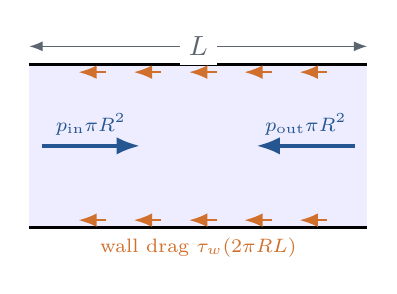
\begin{tikzpicture}[x=0.78cm,y=0.78cm,>=Latex]
  \fill[blue!7] (0,0.6) rectangle (5.5,3.25);
  \draw[very thick] (0,0.6)--(5.5,0.6);
  \draw[very thick] (0,3.25)--(5.5,3.25);
  \draw[->,very thick,pipeblue] (0.2,1.93)--(1.8,1.93) node[midway,above]{\scriptsize $p_{\rm in}\pi R^2$};
  \draw[<-,very thick,pipeblue] (3.7,1.93)--(5.3,1.93) node[midway,above]{\scriptsize $p_{\rm out}\pi R^2$};
  \foreach \x in {0.8,1.7,2.6,3.5,4.4}{
    \draw[<-,pipeorange,thick] (\x,0.72)--(\x+0.45,0.72);
    \draw[<-,pipeorange,thick] (\x,3.13)--(\x+0.45,3.13);
  }
  \node[pipeorange] at (2.75,0.28){\scriptsize wall drag $\tau_w(2\pi RL)$};
  \draw[<->,pipegray] (0,3.55)--(5.5,3.55) node[midway,fill=white]{$L$};
\end{tikzpicture}
\end{column}
\end{columns}
\end{frame}

% ----- 12. Friction factors -----
\begin{frame}{Darcy and Fanning friction factors differ by four}
The Darcy--Weisbach convention is
\[
  \Delta p=f_D\frac LD\frac{\rho U_b^2}{2},
  \qquad
  f_D=\frac{8\tau_w}{\rho U_b^2}.
\]
For Hagen--Poiseuille flow,
\[
  \boxed{f_D=\frac{64}{\Rey_D}}.
\]

The Fanning convention instead defines
\[
  f_F=\frac{\tau_w}{\tfrac12\rho U_b^2}
  =\frac{16}{\Rey_D},
  \qquad f_D=4f_F.
\]

\begin{alertblock}{Notation check}
Always identify the convention: the same symbol $f$ is used for both in the literature.
\end{alertblock}
\end{frame}

% ----- 13. Nondimensionalization -----
\begin{frame}{Nondimensionalization isolates $\Rey_D$}
Choose
\[
  \xvec=D\xvec^*,
  \qquad t=\frac D{U_b}t^*,
  \qquad \uu=U_b\uu^*,
  \qquad p=\rho U_b^2p^*.
\]
After substitution and dropping stars,
\[
  \partial_t\uu+(\uu\cdot\nabla)\uu
  =-\nabla p+\frac1{\Rey_D}\nabla^2\uu,
  \qquad \nabla\cdot\uu=0.
\]

\begin{punchbox}
$\Rey_D=U_bD/\nu$ compares convective inertia with viscous diffusion under this scaling. It is essential, but it is not the only control parameter once forcing, geometry, and wall mechanics vary.
\end{punchbox}
\end{frame}

% ----- 14. Turbulent changes -----
\begin{frame}{Turbulence changes drag and introduces fluctuations}
\begin{columns}[T,onlytextwidth]
\begin{column}{0.49\textwidth}
At \emph{fixed bulk flow rate}, turbulence generally requires a larger pressure gradient than the laminar relation predicts; the friction factor departs from $64/\Rey_D$.

For smooth turbulent pipes the Blasius correlation $f_D\approx0.316\,\Rey_D^{-1/4}$ ($4\times10^3\lesssim\Rey_D\lesssim10^5$) applies; rough pipes follow the Colebrook equation, summarized in the Moody chart.

At fixed pressure gradient, the bulk flow rate instead changes. State what is held fixed.
\end{column}
\begin{column}{0.47\textwidth}
Choose a time, ensemble, or phase average and write
\[
  \uu=\mean{\uu}+\uu',
  \qquad \mean{\uu'}=0.
\]
Although the mean fluctuation vanishes,
\[
  \mean{u_i'u_j'}\ne0
\]
and these correlations alter mean momentum transport.
\end{column}
\end{columns}

\begin{punchbox}
For pulsatile flow, a phase average and a long-time mean answer different questions.
\end{punchbox}
\end{frame}

% ----- 15. DNS resolution -----
\begin{frame}{DNS cost grows after turbulence creates small scales}
\begin{columns}[T,onlytextwidth]
\begin{column}{0.52\textwidth}
Reynolds number alone does not create a turbulent cascade: the flow must first become turbulent.

Once it does,
\begin{itemize}\itemsep4pt
  \item outer structures remain $O(D)$;
  \item dissipative and near-wall scales shrink;
  \item the wall-normal mesh and time step become severe;
  \item wall-resolved cost is often organized by the friction Reynolds number $\Rey_\tau=u_\tau R/\nu$, with friction velocity $u_\tau=\sqrt{\tau_w/\rho}$.
\end{itemize}
\soft{Exact cost scaling depends on domain, numerics, and what is resolved.}
\end{column}
\begin{column}{0.45\textwidth}
\centering
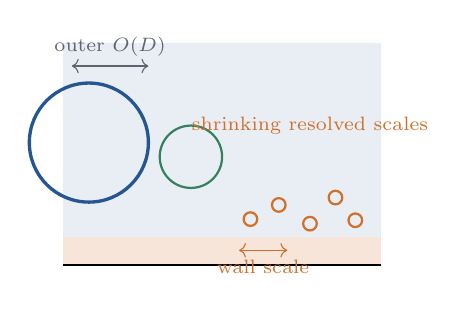
\begin{tikzpicture}[x=0.72cm,y=0.72cm]
  \draw[very thick] (0,0)--(5.6,0);
  \fill[pipeorange!18] (0,0) rectangle (5.6,0.48);
  \fill[pipeblue!10] (0,0.48) rectangle (5.6,3.9);
  \draw[pipeblue,very thick] (0.45,2.15) circle (1.05);
  \draw[pipegreen,thick] (2.25,1.9) circle (0.55);
  \foreach \x/\y in {3.3/0.8,3.8/1.05,4.35/0.72,4.8/1.18,5.15/0.78}{
    \draw[pipeorange,thick] (\x,\y) circle (0.12);
  }
  \draw[<->,pipegray] (0.15,3.5)--(1.5,3.5) node[midway,above]{\scriptsize outer $O(D)$};
  \draw[<->,pipeorange] (3.1,0.25)--(3.95,0.25) node[midway,below]{\scriptsize wall scale};
  \node[pipeorange] at (4.35,2.45){\scriptsize shrinking resolved scales};
\end{tikzpicture}
\end{column}
\end{columns}
\end{frame}

% ----- 16. Modal stability -----
\begin{frame}{Pipe transition has no known modal instability}
\begin{columns}[T,onlytextwidth]
\begin{column}{0.56\textwidth}
Fully developed Hagen--Poiseuille flow is eigenvalue stable in all computations to date. Meseguer and Trefethen computed a stable linearized spectrum through
\[
  \Rey_D=10^7.
\]
Yet finite disturbances can trigger turbulence at far lower Reynolds numbers.

\begin{block}{Subcritical transition}
Infinitesimal eigenmodes decay, but finite-amplitude perturbations, transient amplification, and nonlinear feedback can produce turbulent dynamics.
\end{block}
\end{column}
\begin{column}{0.41\textwidth}
\centering
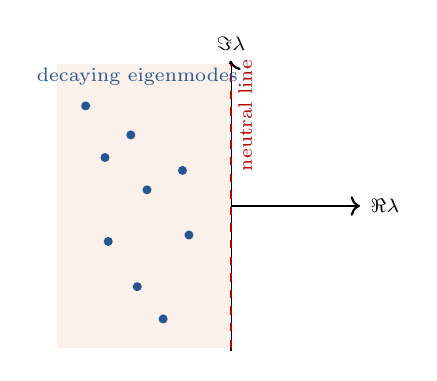
\begin{tikzpicture}[x=0.82cm,y=0.82cm]
  \draw[->,thick] (-2.7,0)--(2.0,0) node[right]{\scriptsize $\Re\lambda$};
  \draw[->,thick] (0,-2.25)--(0,2.25) node[above]{\scriptsize $\Im\lambda$};
  \fill[pipeorange!10] (-2.7,-2.2) rectangle (0,2.2);
  \foreach \x/\y in {-2.25/1.55,-1.95/0.75,-1.55/1.1,-1.3/0.25,-1.9/-0.55,-1.45/-1.25,-0.75/0.55,-0.65/-0.45,-1.05/-1.75}{
    \fill[pipeblue] (\x,\y) circle (0.07);
  }
  \draw[red!70!black,dashed,thick] (0,-2.2)--(0,2.2);
  \node[pipeblue] at (-1.45,2.0){\scriptsize decaying eigenmodes};
  \node[red!70!black,rotate=90] at (0.22,1.4){\scriptsize neutral line};
\end{tikzpicture}

\vspace{0.3em}
{\scriptsize \href{https://doi.org/10.1016/S0021-9991(03)00029-9}{Meseguer \& Trefethen (2003)}}
\end{column}
\end{columns}
\end{frame}

% ----- 17. Perturbation equation -----
\begin{frame}{Perturb about the Poiseuille base state}
Let $\uu=U(r)\bm e_z+\widetilde{\uu}$. The nondimensional perturbation equation is
\begin{align*}
  \partial_t\widetilde{\uu}
  &+U\partial_z\widetilde{\uu}
  +\widetilde u_rU'(r)\bm e_z
  +(\widetilde{\uu}\cdot\nabla)\widetilde{\uu}\\
  &=-\nabla\widetilde p+\frac1{\Rey_D}\nabla^2\widetilde{\uu},
  \qquad \nabla\cdot\widetilde{\uu}=0.
\end{align*}

\begin{itemize}\itemsep3pt
  \item Linear dynamics include base advection, shear coupling, pressure, and viscosity.
  \item The quadratic term redistributes energy among perturbation modes.
  \item Use $\widetilde{\uu}=0$ at $r=R$ and periodic or suitably decaying conditions in $z$.
\end{itemize}

\begin{alertblock}{Three different tildes and primes}
Here $\widetilde{\uu}$ is a \emph{deterministic} perturbation about a specified base state, not the turbulent fluctuation $\uu'$ of the Reynolds decomposition (a statistical deviation from an average, as on the turbulence slide), and not the LES filtered field $\widetilde{\uu}$ of deck 5-3 (a spatially coarse-grained field). Same symbols, three different meanings.
\end{alertblock}
\end{frame}

% ----- 18. Non-normality -----
\begin{frame}{Non-normality permits transient growth}
For the linearized system $\partial_t\qv=L\qv$,
\[
  L^*L\ne LL^*,
  \qquad
  G(t):=\max_{\qv_0\ne0}
  \frac{\|e^{tL}\qv_0\|_E^2}{\|\qv_0\|_E^2}.
\]
Stable eigenvalues do not require $G(t)$ to decrease monotonically.

\begin{columns}[T,onlytextwidth]
\begin{column}{0.48\textwidth}
\begin{block}{High-$\Rey_D$ scaling}
For the optimal streamwise-constant, azimuthal-$n=1$ mechanism, velocity amplification is $O(\Rey_D)$ and energy gain is $O(\Rey_D^2)$.
\end{block}
\end{column}
\begin{column}{0.48\textwidth}
\centering
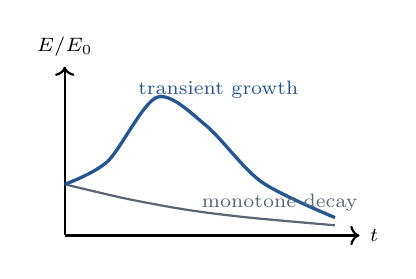
\begin{tikzpicture}[x=0.78cm,y=0.65cm]
  \draw[->,thick] (0,0)--(4.8,0) node[right]{\scriptsize $t$};
  \draw[->,thick] (0,0)--(0,3.3) node[above]{\scriptsize $E/E_0$};
  \draw[pipegray,thick] plot[smooth] coordinates{(0,1)(1,0.72)(2,0.5)(3,0.35)(4.4,0.2)};
  \draw[pipeblue,very thick] plot[smooth] coordinates{(0,1)(0.7,1.45)(1.5,2.7)(2.3,2.15)(3.2,1.05)(4.4,0.35)};
  \node[pipegray] at (3.5,0.65){\scriptsize monotone decay};
  \node[pipeblue] at (2.5,2.85){\scriptsize transient growth};
\end{tikzpicture}
\end{column}
\end{columns}
\soft{Transient growth is an amplification mechanism, not by itself a transition criterion.}
\end{frame}

% ----- 19. Lift-up -----
\begin{frame}{Lift-up converts cross-stream motion into streaks}
\begin{columns}[T,onlytextwidth]
\begin{column}{0.50\textwidth}
Weak streamwise vortices move low-speed fluid away from the wall and high-speed fluid toward it. The base shear then creates large streamwise velocity streaks.

\begin{itemize}\itemsep4pt
  \item cross-stream velocity can remain small;
  \item the induced streamwise perturbation can grow algebraically;
  \item nonlinear feedback is needed to regenerate the rolls and sustain turbulence.
\end{itemize}
\end{column}
\begin{column}{0.47\textwidth}
\centering
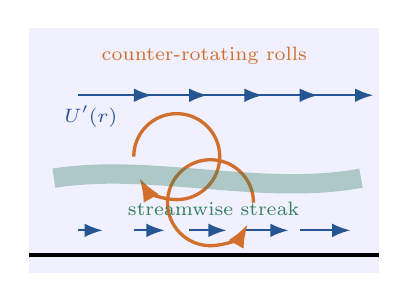
\begin{tikzpicture}[x=0.78cm,y=0.78cm,>=Latex]
  \fill[blue!6] (0,0) rectangle (5.7,4.0);
  \draw[very thick] (0,0.3)--(5.7,0.3);
  \foreach \x in {0.8,1.7,2.6,3.5,4.4}{
    \draw[->,pipeblue,thick] (\x,0.7)--(\x+0.3+0.12*\x,0.7);
    \draw[->,pipeblue,thick] (\x,2.9)--(\x+1.2,2.9);
  }
  \draw[pipeorange,very thick,->] (1.7,1.9) arc[start angle=180,end angle=-150,radius=0.7];
  \draw[pipeorange,very thick,->] (3.65,1.15) arc[start angle=0,end angle=330,radius=0.7];
  \draw[pipegreen,line width=7pt,opacity=0.35] (0.4,1.55) .. controls (2.0,1.8) and (3.8,1.25) .. (5.4,1.55);
  \node[pipeorange] at (2.85,3.55){\scriptsize counter-rotating rolls};
  \node[pipegreen] at (3.0,1.05){\scriptsize streamwise streak};
  \node[pipeblue] at (1.0,2.55){\scriptsize $U'(r)$};
\end{tikzpicture}
\end{column}
\end{columns}
\end{frame}

% ----- 20. Energy method -----
\begin{frame}{The perturbation-energy budget isolates mean-shear extraction}
Let
\[
  E(t)=\frac12\int_\Omega|\widetilde{\uu}|^2\,\mathrm dV.
\]
With no slip at the wall and periodic or suitably decaying axial conditions,
\[
  \frac{\mathrm dE}{\mathrm dt}
  =-\int_\Omega \widetilde u_z\widetilde u_rU'(r)\,\mathrm dV
   -\frac1{\Rey_D}\int_\Omega|\nabla\widetilde{\uu}|^2\,\mathrm dV.
\]

\begin{columns}[T,onlytextwidth]
\begin{column}{0.48\textwidth}
The first term is signed production from the base shear; the second is nonnegative viscous dissipation.
\end{column}
\begin{column}{0.48\textwidth}
The nonlinear perturbation term redistributes energy but contributes zero to the net integral under these conditions.
\end{column}
\end{columns}

\soft{Above an energy-stability bound, the estimate becomes inconclusive; it does not prove transition.}
\end{frame}

% ----- 21. Edge dynamics -----
\begin{frame}{Finite-amplitude outcomes motivate an ``edge'' picture}
\begin{columns}[T,onlytextwidth]
\begin{column}{0.51\textwidth}
At a fixed Reynolds number and observation protocol:
\begin{itemize}\itemsep4pt
  \item sufficiently small disturbances return to laminar flow;
  \item some larger disturbances visit long-lived turbulent dynamics;
  \item a complicated state-space boundary separates these outcomes.
\end{itemize}

\begin{block}{Scope of the picture}
In a finite or open pipe, ``sustained'' depends on domain length, forcing, and observation time. The edge is a dynamical-systems idealization, not a universal amplitude threshold.
\end{block}
\end{column}
\begin{column}{0.46\textwidth}
\centering
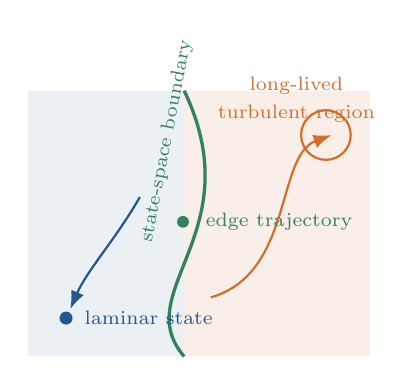
\begin{tikzpicture}[x=0.75cm,y=0.75cm,>=Latex]
  \fill[pipeblue!9] (0,0) rectangle (2.65,4.5);
  \fill[pipeorange!11] (2.65,0) rectangle (5.8,4.5);
  \draw[pipegreen,very thick] (2.65,0) .. controls (1.7,1.1) and (3.8,2.1) .. (2.65,4.5);
  \fill[pipeblue] (0.65,0.65) circle (0.11);
  \node[pipeblue,anchor=west] at (0.8,0.65){\scriptsize laminar state};
  \draw[->,pipeblue,thick] (1.9,2.7) .. controls (1.5,2.0) and (1.0,1.45) .. (0.72,0.8);
  \draw[->,pipeorange,thick] (3.1,1.0) .. controls (4.5,1.4) and (4.2,3.4) .. (5.15,3.75);
  \draw[pipeorange,thick] (5.05,3.75) circle (0.42);
  \node[pipeorange,align=center] at (4.55,4.35){\scriptsize long-lived\\[-2pt]\scriptsize turbulent region};
  \fill[pipegreen] (2.63,2.28) circle (0.10);
  \node[pipegreen,anchor=west] at (2.85,2.28){\scriptsize edge trajectory};
  \node[pipegreen,rotate=79] at (2.35,3.65){\scriptsize state-space boundary};
\end{tikzpicture}
\end{column}
\end{columns}
\end{frame}

% ----- 22. Reynolds experiment -----
\begin{frame}{Reynolds' dye experiment also measures disturbance sensitivity}
\begin{columns}[T,onlytextwidth]
\begin{column}{0.48\textwidth}
At low $\Rey_D$, a carefully introduced filament can remain coherent. With larger Reynolds number or larger inlet disturbance, it breaks down and mixes.

\begin{itemize}\itemsep4pt
  \item transition is not specified by $\Rey_D$ alone;
  \item inlet quality, disturbance shape, pipe length, and observation time matter;
  \item deliberately triggered and naturally occurring transition should be distinguished.
\end{itemize}
\end{column}
\begin{column}{0.49\textwidth}
\centering
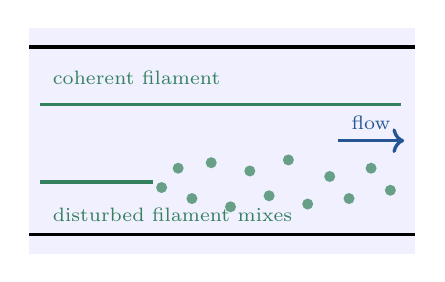
\begin{tikzpicture}[x=0.70cm,y=0.70cm]
  \fill[blue!6] (0,0) rectangle (7.0,4.1);
  \draw[very thick] (0,0.35)--(7,0.35);
  \draw[very thick] (0,3.75)--(7,3.75);
  \draw[pipegreen,very thick] (0.2,2.7)--(6.75,2.7);
  \node[pipegreen,anchor=west] at (0.25,3.2){\scriptsize coherent filament};
  \draw[pipegreen,very thick] (0.2,1.3)--(2.25,1.3);
  \foreach \x/\y in {2.4/1.2,2.7/1.55,2.95/1.0,3.3/1.65,3.65/0.85,4.0/1.5,4.35/1.05,4.7/1.7,5.05/0.9,5.45/1.4,5.8/1.0,6.2/1.55,6.55/1.15}{
    \fill[pipegreen!75] (\x,\y) circle (0.10);
  }
  \node[pipegreen,anchor=west] at (0.25,0.7){\scriptsize disturbed filament mixes};
  \draw[->,pipeblue,very thick] (5.6,2.05)--(6.8,2.05) node[midway,above]{\scriptsize flow};
\end{tikzpicture}

\vspace{0.3em}
{\scriptsize \href{https://doi.org/10.1098/rstl.1883.0029}{Reynolds (1883)}}
\end{column}
\end{columns}
\end{frame}

% ----- 23. Puff anatomy -----
\begin{frame}{A puff is localized---not immortal}
\begin{columns}[T,onlytextwidth]
\begin{column}{0.48\textwidth}
A puff is a localized turbulent patch in the lower transitional range.
\begin{itemize}\itemsep4pt
  \item sharp upstream/trailing interface;
  \item diffuse downstream/leading recovery region;
  \item travels near the bulk velocity;
  \item remains approximately localized while it exists.
\end{itemize}

An individual puff can decay stochastically; ``persistent'' should not mean infinite lifetime.
\end{column}
\begin{column}{0.49\textwidth}
\centering
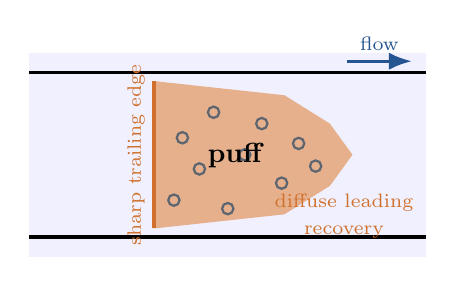
\begin{tikzpicture}[x=0.72cm,y=0.72cm,>=Latex]
  \fill[blue!6] (0,0) rectangle (7,3.6);
  \draw[very thick] (0,0.35)--(7,0.35);
  \draw[very thick] (0,3.25)--(7,3.25);
  \fill[pipeorange!55] (2.2,0.5) -- (2.2,3.1) -- (4.5,2.85) -- (5.3,2.35) -- (5.7,1.8) -- (5.3,1.25) -- (4.5,0.75) -- cycle;
  \draw[pipeorange,very thick] (2.2,0.5)--(2.2,3.1);
  \foreach \x/\y in {2.55/1.0,2.7/2.1,3.0/1.55,3.25/2.55,3.5/0.85,3.8/1.8,4.1/2.35,4.45/1.3,4.75/2.0,5.05/1.6}{
    \draw[pipegray,thick] (\x,\y) circle (0.10);
  }
  \draw[->,pipeblue,very thick] (5.6,3.45)--(6.75,3.45) node[midway,above]{\scriptsize flow};
  \node[pipeorange,rotate=90] at (1.88,1.8){\scriptsize sharp trailing edge};
  \node[pipeorange,align=center] at (5.55,0.72){\scriptsize diffuse leading\\[-2pt]\scriptsize recovery};
  \node at (3.65,1.78){\textbf{puff}};
\end{tikzpicture}
\end{column}
\end{columns}
\end{frame}

% ----- 24. Slug anatomy -----
\begin{frame}{A slug grows because its two fronts have different speeds}
\begin{columns}[T,onlytextwidth]
\begin{column}{0.49\textwidth}
A turbulent slug has identifiable leading and trailing fronts. In the laboratory frame, both fronts normally advect downstream, but
\[
  c_{\rm lead}>c_{\rm trail}
\]
so the turbulent region lengthens.

\begin{alertblock}{Wording to avoid}
``The slug propagates upstream'' confuses growth relative to the fluid with absolute front motion.
\end{alertblock}

Puffs and slugs describe different transitional regimes, not merely different drawing styles.
\end{column}
\begin{column}{0.48\textwidth}
\centering
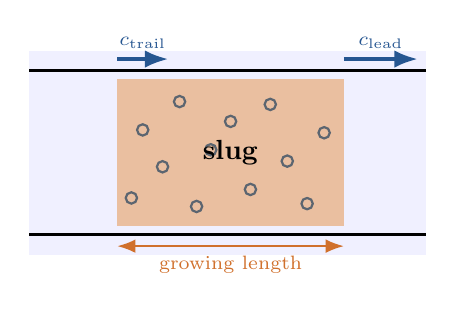
\begin{tikzpicture}[x=0.72cm,y=0.72cm,>=Latex]
  \fill[blue!6] (0,0) rectangle (7,3.6);
  \draw[very thick] (0,0.35)--(7,0.35);
  \draw[very thick] (0,3.25)--(7,3.25);
  \fill[pipeorange!45] (1.55,0.5) rectangle (5.55,3.1);
  \foreach \x/\y in {1.8/1.0,2.0/2.2,2.35/1.55,2.65/2.7,2.95/0.85,3.2/1.85,3.55/2.35,3.9/1.15,4.25/2.65,4.55/1.65,4.9/0.9,5.2/2.15}{
    \draw[pipegray,thick] (\x,\y) circle (0.10);
  }
  \draw[->,very thick,pipeblue] (1.55,3.45)--(2.45,3.45) node[midway,above]{\scriptsize $c_{\rm trail}$};
  \draw[->,very thick,pipeblue] (5.55,3.45)--(6.85,3.45) node[midway,above]{\scriptsize $c_{\rm lead}$};
  \draw[<->,pipeorange,thick] (1.55,0.15)--(5.55,0.15) node[midway,below]{\scriptsize growing length};
  \node at (3.55,1.8){\textbf{slug}};
\end{tikzpicture}

\vspace{0.25em}
{\scriptsize Anatomy and front behavior: \href{https://doi.org/10.1017/S0022112073001576}{Wygnanski \& Champagne (1973)}.}
\end{column}
\end{columns}
\end{frame}

% ----- 25. Puff statistics -----
\begin{frame}{Puff decay and splitting are competing stochastic events}
Measure two conditional times at fixed $\Rey_D$ and disturbance protocol:
\[
  \tau_{\rm decay}(\Rey_D),
  \qquad
  \tau_{\rm split}(\Rey_D).
\]

\begin{columns}[T,onlytextwidth]
\begin{column}{0.48\textwidth}
\begin{block}{Decay dominates}
If splitting is slower than decay, turbulent patches disappear in the long-pipe, long-time limit.
\end{block}
\end{column}
\begin{column}{0.48\textwidth}
\begin{block}{Splitting dominates}
If splitting is faster, new puffs can maintain a nonzero turbulent fraction even though each puff remains mortal.
\end{block}
\end{column}
\end{columns}

Avila et al. measured a balance at
\[
  \boxed{\Rey_D=2040\pm10.}
\]
This is a statistical onset of sustained turbulence, not an immortality threshold for one puff.
The textbook value $\Rey_D\approx2300$ marks practical onset of transition; $2040$ is the statistically defined point where puff splitting balances decay.
\end{frame}

% ----- 26. Spacetime -----
\begin{frame}{A space--time diagram reveals propagation, decay, and splitting}
\begin{columns}[T,onlytextwidth]
\begin{column}{0.47\textwidth}
Horizontal position is $z$; time increases upward. The slope of each interface encodes a front speed.

\begin{itemize}\itemsep4pt
  \item a band ending in time is puff decay;
  \item one band branching into two is splitting;
  \item widening separation between fronts is slug growth;
  \item turbulent fraction becomes a spatiotemporal statistic.
\end{itemize}
\end{column}
\begin{column}{0.50\textwidth}
\centering
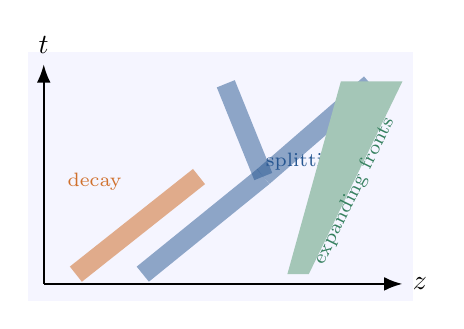
\begin{tikzpicture}[x=0.68cm,y=0.62cm,>=Latex]
  \fill[blue!4] (0,0) rectangle (7.2,5.1);
  \draw[->,thick] (0.3,0.35)--(7.0,0.35) node[right]{$z$};
  \draw[->,thick] (0.3,0.35)--(0.3,4.85) node[above]{$t$};
  \draw[pipeorange,line width=7pt,opacity=0.55] (0.9,0.55)--(3.2,2.55);
  \node[pipeorange] at (1.25,2.45){\scriptsize decay};
  \draw[pipeblue,line width=7pt,opacity=0.50] (2.15,0.55)--(4.4,2.55);
  \draw[pipeblue,line width=7pt,opacity=0.50] (4.4,2.55)--(6.4,4.45);
  \draw[pipeblue,line width=7pt,opacity=0.50] (4.4,2.55)--(3.7,4.45);
  \node[pipeblue] at (5.2,2.85){\scriptsize splitting};
  \fill[pipegreen!45] (4.85,0.55)--(5.25,0.55)--(7.0,4.5)--(5.85,4.5)--cycle;
  \node[pipegreen,rotate=64] at (6.1,2.25){\scriptsize expanding fronts};
\end{tikzpicture}

{\scriptsize Critical balance: \href{https://doi.org/10.1126/science.1203223}{Avila et al. (2011)}.}
\end{column}
\end{columns}
\end{frame}

% ----- 27. Observables -----
\begin{frame}{Transition observables need a conditioning statement}
Useful measurements include
\begin{itemize}\itemsep5pt
  \item puff decay and splitting time distributions;
  \item leading/trailing front speeds and turbulent fraction;
  \item probability of relaminarization over a stated observation window;
  \item friction-factor departure from $64/\Rey_D$;
  \item velocity variance, Reynolds stresses, spectra, and wall-shear statistics.
\end{itemize}

For smooth turbulent pipes the Blasius correlation $f_D\approx0.316\,\Rey_D^{-1/4}$ ($4\times10^3\lesssim\Rey_D\lesssim10^5$) applies; rough pipes follow the Colebrook equation, summarized in the Moody chart.

\begin{punchbox}
Report $\Rey_D$, pipe length, inlet/disturbance protocol, boundary conditions, and observation time. One finite run cannot establish ``sustained forever.''
\end{punchbox}

For cardiovascular flow, connect each statistic to pressure loss, wall loading, mixing, or another biomechanical quantity of interest.
\end{frame}

% ----- 28. Pipe-to-aorta bridge -----
\begin{frame}{The pipe-to-aorta analogy names mechanisms, not thresholds}
\begin{columns}[T,onlytextwidth]
\begin{column}{0.47\textwidth}
\begin{block}{What transfers}
\begin{itemize}\itemsep3pt
  \item inertia--viscosity competition;
  \item shear production and transient growth;
  \item disturbance sensitivity;
  \item intermittency and front dynamics.
\end{itemize}
\end{block}
\end{column}
\begin{column}{0.49\textwidth}
\begin{alertblock}{What changes}
\begin{itemize}\itemsep3pt
  \item periodic acceleration/deceleration;
  \item curvature, branches, entrance jets, taper;
  \item moving compliant walls and pressure waves;
  \item finite length and patient-specific inflow.
\end{itemize}
\end{alertblock}
\end{column}
\end{columns}

\vspace{0.45em}
\hi{Consequence:} a steady straight-pipe transition Reynolds number cannot be imported as an aortic turbulence criterion.
\end{frame}

% ----- 29. Womersley -----
\begin{frame}{Womersley number compares unsteadiness with viscous diffusion}
\begin{columns}[T,onlytextwidth]
\begin{column}{0.56\textwidth}
For angular frequency $\omega$,
\[
  \alpha=R\sqrt{\frac{\omega}{\nu}}
  =R\sqrt{\frac{\omega\rho}{\mu}}.
\]
The oscillatory Stokes-layer thickness is
\[
  \delta_s=\sqrt{\frac{2\nu}{\omega}},
  \qquad \frac{\delta_s}{R}=\frac{\sqrt2}{\alpha}.
\]
If $\mathrm{St}_\omega=\omega D/U_b$, then
\[
  \alpha^2=\frac{\Rey_D\mathrm{St}_\omega}{4}.
\]
\soft{Large $\alpha$ means a thinner oscillatory wall layer and stronger phase lag; it does not imply turbulence.}
\end{column}
\begin{column}{0.41\textwidth}
\centering
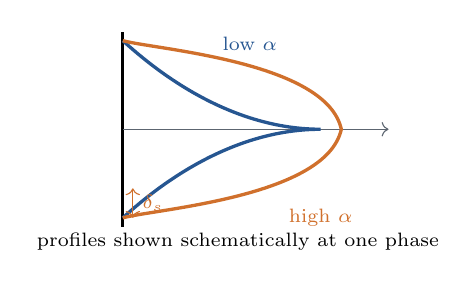
\begin{tikzpicture}[x=0.75cm,y=0.75cm]
  \draw[very thick] (0.45,0.3)--(0.45,3.6);
  \draw[->,pipegray] (0.45,1.95)--(4.95,1.95);
  \draw[pipeblue,very thick] (0.45,0.45) parabola bend (3.8,1.95) (0.45,3.45);
  \node[pipeblue] at (2.6,3.4){\scriptsize low $\alpha$};
  \draw[pipeorange,very thick] (0.45,0.45) .. controls (1.0,0.6) and (3.9,0.8) .. (4.15,1.95)
     .. controls (3.9,3.1) and (1.0,3.3) .. (0.45,3.45);
  \node[pipeorange] at (3.8,0.45){\scriptsize high $\alpha$};
  \draw[<->,pipeorange] (0.62,0.45)--(0.62,0.95) node[midway,right]{\scriptsize $\delta_s$};
  \node[align=center] at (2.4,0.05){\scriptsize profiles shown schematically at one phase};
\end{tikzpicture}

\vspace{0.25em}
{\scriptsize \href{https://doi.org/10.1113/jphysiol.1955.sp005276}{Womersley (1955)}}
\end{column}
\end{columns}
\end{frame}

% ----- 30. Pulsatile transition -----
\begin{frame}{Pulsatile transition occupies a multi-parameter space}
\centering
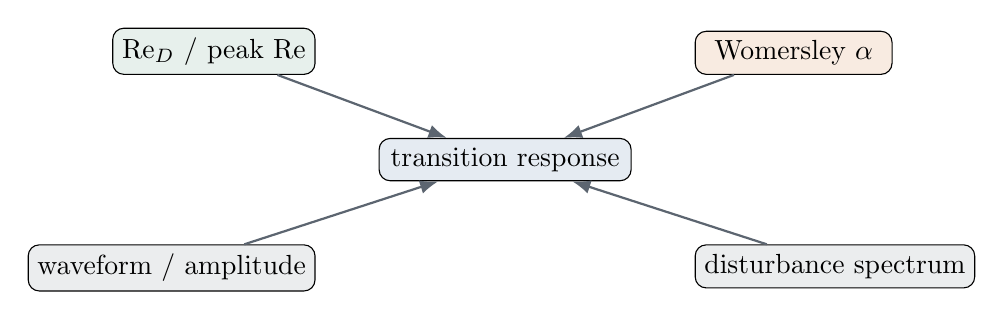
\begin{tikzpicture}[node distance=0.55cm and 0.55cm,>=Latex]
  \node[draw,rounded corners,fill=pipeblue!12,minimum width=3.2cm] (trans) {transition response};
  \node[draw,rounded corners,fill=pipegreen!12,above left=0.8cm and 0.8cm of trans,minimum width=2.5cm] (re) {$\Rey_D$ / peak $\Rey$};
  \node[draw,rounded corners,fill=pipeorange!14,above right=0.8cm and 0.8cm of trans,minimum width=2.5cm] (alpha) {Womersley $\alpha$};
  \node[draw,rounded corners,fill=pipegray!12,below left=0.8cm and 0.8cm of trans,minimum width=2.5cm] (wave) {waveform / amplitude};
  \node[draw,rounded corners,fill=pipegray!12,below right=0.8cm and 0.8cm of trans,minimum width=2.5cm] (dist) {disturbance spectrum};
  \draw[->,thick,pipegray] (re)--(trans);
  \draw[->,thick,pipegray] (alpha)--(trans);
  \draw[->,thick,pipegray] (wave)--(trans);
  \draw[->,thick,pipegray] (dist)--(trans);
\end{tikzpicture}

\vspace{0.8em}
Acceleration, deceleration, and flow reversal can change the base profile and its receptivity throughout a cycle. A phase-resolved stability or simulation analysis must specify the waveform and disturbance.

\begin{punchbox}
\centering
Neither high peak Reynolds number nor large Womersley number alone is a turbulence criterion.
\end{punchbox}
\end{frame}

% ----- 31. Curvature -----
\begin{frame}{Curvature introduces secondary flow; branching is different}
\small
\begin{columns}[T,onlytextwidth]
\begin{column}{0.54\textwidth}
With centerline radius of curvature $R_c$, define
\[
  \delta_c=\frac R{R_c}=\frac D{2R_c},
  \qquad
  \De=\Rey_D\sqrt{\delta_c}.
\]
The curvature ratio is written $\delta_c$, not $\kappa$, because $\kappa$ is reserved for the von K\'arm\'an constant. This diameter-based convention for $\delta_c$ must be stated because alternatives exist.

In a simple steady laminar curved pipe, centrifugal effects can drive a counter-rotating Dean-vortex pair. Finite curvature, torsion, pulsatility, and wall motion add parameters.

\begin{alertblock}{Branching caveat}
A branch-induced jet or separation zone is not a Dean vortex.
\end{alertblock}
\end{column}
\begin{column}{0.43\textwidth}
\centering
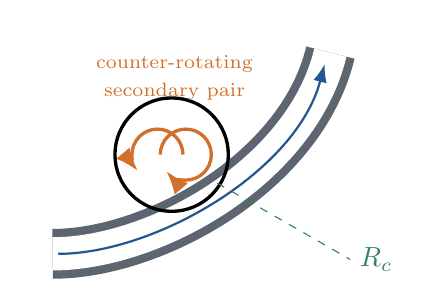
\begin{tikzpicture}[x=0.72cm,y=0.72cm,>=Latex]
  \draw[pipegray,line width=18pt] (0.3,0.45) .. controls (2.1,0.45) and (4.7,1.9) .. (5.2,4.0);
  \draw[white,line width=12pt] (0.3,0.45) .. controls (2.1,0.45) and (4.7,1.9) .. (5.2,4.0);
  \draw[pipeblue,thick,->] (0.4,0.45) .. controls (2.1,0.45) and (4.6,1.9) .. (5.1,3.8);
  \draw[very thick] (2.4,2.2) circle (1.0);
  \draw[pipeorange,very thick,->] (2.2,2.2) arc[start angle=180,end angle=-140,radius=0.45];
  \draw[pipeorange,very thick,->] (2.6,2.2) arc[start angle=0,end angle=220,radius=0.45];
  \node[pipeorange,align=center] at (2.45,3.55){\scriptsize counter-rotating\\[-2pt]\scriptsize secondary pair};
  \draw[dashed,pipegreen] (3.2,1.7)--(5.55,0.35) node[right]{$R_c$};
\end{tikzpicture}

\vspace{0.2em}
{\scriptsize \href{https://doi.org/10.1080/14786440708564324}{Dean (1927)}}
\end{column}
\end{columns}
\end{frame}

% ----- 32. Compliance -----
\begin{frame}{Compliance adds wave propagation; inflow sets disturbance amplitude}
\small
\begin{columns}[T,onlytextwidth]
\begin{column}{0.49\textwidth}
For normalized area distensibility
\[
  \mathcal D_A=\frac1A\frac{\mathrm dA}{\mathrm dp},
  \qquad
  c=\frac1{\sqrt{\rho\mathcal D_A}}.
\]
This is the \hi{Bramwell--Hill} relation (Bramwell \& Hill 1922, \emph{Proc.\ R. Soc.\ B} \textbf{93}, 298).
A thin, linearly elastic, untethered tube gives the \hi{Moens--Korteweg} scale (Moens 1878; Korteweg 1878)
\[
  c_0\approx\sqrt{\frac{Eh}{\rho D}},
  \qquad \frac{U_b}{c_0}
\]
for convective speed relative to wave speed.
\end{column}
\begin{column}{0.47\textwidth}
Real arteries are prestressed, tethered, anisotropic, viscoelastic, and nonlinear. The specified FSI model determines whether compliance amplifies or attenuates a disturbance.

Valve jets, swirl, upstream turbulence, and phase-dependent inlet profiles set finite-amplitude perturbations that a subcritical system can amplify.
\end{column}
\end{columns}

\begin{punchbox}
\centering
State the wall law and inlet condition before making a stability claim.
\end{punchbox}
\end{frame}

% ----- 33. Modeling map -----
\begin{frame}{Choose a model by resolved physics and quantity of interest}
\small
\setlength{\tabcolsep}{3pt}
\begin{tabular}{@{}L{0.16\textwidth}L{0.24\textwidth}L{0.24\textwidth}L{0.27\textwidth}@{}}
\toprule
\textbf{Method} & \textbf{Resolved field} & \textbf{Key modeling} & \textbf{Aortic question}\\
\midrule
DNS & all dynamically relevant scales & geometry, wall, inflow & reference cases; mechanism discovery\\[3pt]
LES & large unsteady eddies & SGS, wall, inflow, FSI & jets, wakes, mixing, fluctuation statistics\\[3pt]
RANS/URANS & mean or phase-resolved mean & Reynolds stress, wall, transition & design sweeps; mean pressure and shear\\[3pt]
Hybrid & RANS region plus resolved eddies & grid/model interface, wall & high-$\Rey$ separated regions\\
\bottomrule
\end{tabular}

\vspace{0.65em}
\begin{punchbox}
There is no universal accuracy ordering. Grid resolution, wall treatment, inflow data, FSI assumptions, and validation against the chosen output all matter.
\end{punchbox}
\end{frame}

% ----- 34. Takeaways -----
\begin{frame}{Takeaways: carry conventions and caveats forward}
\begin{itemize}\itemsep5pt
  \item Hagen--Poiseuille flow links $\Delta p$, $Q$, $U_b$, and the \emph{positive} wall-shear magnitude $\tau_w$; Darcy and Fanning factors differ by four.
  \item Fully developed pipe flow has no known modal instability, yet non-normal growth can amplify finite disturbances before nonlinear feedback acts.
  \item Puffs can decay or split; sustained turbulence is a statistical population balance, not an immortal-puff threshold.
  \item Large $\Rey_D$ or $\alpha$ alone does not establish turbulence in a pulsatile flow.
  \item Curvature, branching, compliance, and inlet disturbances require explicit additional parameters and models.
\end{itemize}

\begin{punchbox}
\centering
The pipe is the clean control problem; the aorta is a time-dependent fluid--structure system.
\end{punchbox}
\end{frame}

% ----- 35. References -----
\begin{frame}{Primary references}
\scriptsize
\begin{itemize}\itemsep4pt
  \item O. Reynolds, ``An experimental investigation of the circumstances which determine whether the motion of water shall be direct or sinuous,'' \emph{Phil. Trans. R. Soc.} 174 (1883), 935--982. \href{https://doi.org/10.1098/rstl.1883.0029}{doi:10.1098/rstl.1883.0029}.
  \item I. J. Wygnanski and F. H. Champagne, ``On transition in a pipe. Part 1. The origin of puffs and slugs and the flow in a turbulent slug,'' \emph{J. Fluid Mech.} 59 (1973), 281--335. \href{https://doi.org/10.1017/S0022112073001576}{doi:10.1017/S0022112073001576}.
  \item A. Meseguer and L. N. Trefethen, ``Linearized pipe flow to Reynolds number $10^7$,'' \emph{J. Comput. Phys.} 186 (2003), 178--197. \href{https://doi.org/10.1016/S0021-9991(03)00029-9}{doi:10.1016/S0021-9991(03)00029-9}.
  \item K. Avila et al., ``The onset of turbulence in pipe flow,'' \emph{Science} 333 (2011), 192--196. \href{https://doi.org/10.1126/science.1203223}{doi:10.1126/science.1203223}.
  \item J. R. Womersley, ``Method for the calculation of velocity, rate of flow and viscous drag in arteries when the pressure gradient is known,'' \emph{J. Physiol.} 127 (1955), 553--563. \href{https://doi.org/10.1113/jphysiol.1955.sp005276}{doi:10.1113/jphysiol.1955.sp005276}.
  \item J. C. Bramwell and A. V. Hill, ``The velocity of the pulse wave in man,'' \emph{Proc.\ R. Soc.\ B} 93 (1922), 298--306.
  \item A. I. Moens, \emph{Die Pulscurve} (1878); D. J. Korteweg, ``\"Uber die Fortpflanzungsgeschwindigkeit des Schalles in elastischen R\"ohren,'' \emph{Ann.\ Phys.} 241 (1878), 525--542.
  \item W. R. Dean, ``Note on the motion of fluid in a curved pipe,'' \emph{Philosophical Magazine} 4 (1927), 208--223. \href{https://doi.org/10.1080/14786440708564324}{doi:10.1080/14786440708564324}.
\end{itemize}
\end{frame}

\end{document}
